\documentclass[a4paper]{report}
\usepackage[utf8]{inputenc}
\usepackage{amsmath}
\usepackage{standalone}
\usepackage{graphicx}
\usepackage{hyperref}
\usepackage{caption}
\usepackage[colorinlistoftodos]{todonotes} %\todo, \missingfigure
\usepackage[norsk]{babel}
\usepackage{units}
\usepackage{float}
\usepackage[amssymb]{SIunits}
\usepackage{placeins} %To use \FloatBarrier
\newcommand{\tab}[1]{\hspace{.2\textwidth}\rlap{#1}}
\usepackage[parfill]{parskip}

%-----------------------------------------------------------------

\begin{document}
\todo{Find info from here: \url{http://sharki.oslo.dnmi.no/portal/page?_pageid=73,39035,73_39049&_dad=portal&_schema=PORTAL}}

\chapter{Teori}

\todo{Research Weibul distribution}
\section{Wind Turbine}
At Racco wind farm they have installed 15 Siemens SWT-101 3.0MW turbines.
\begin{figure}
    \centering
    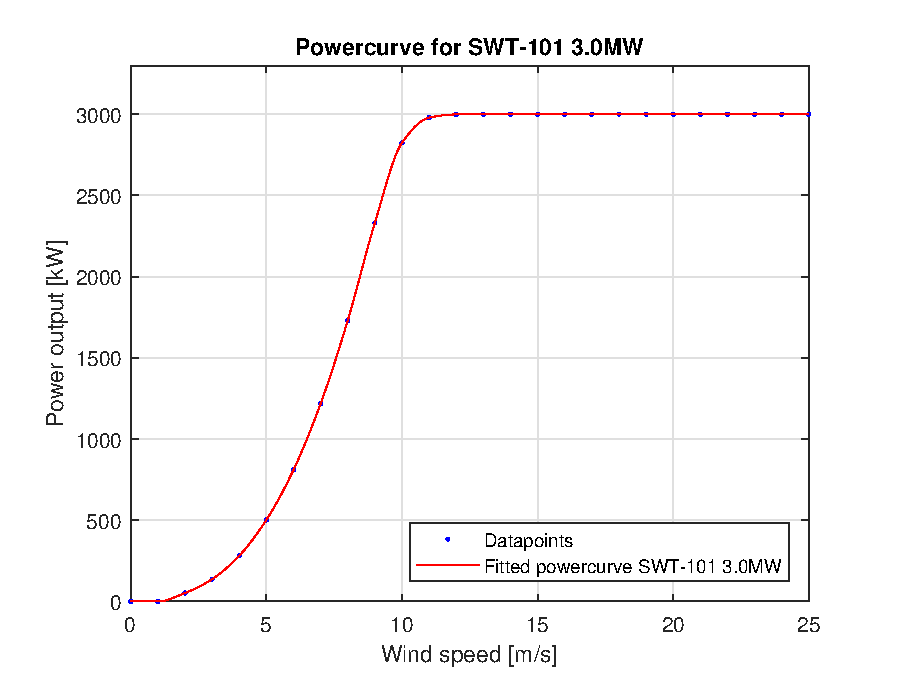
\includegraphics{Theory/figures/PowerCurve}
    \caption{Powercurve-fitting of the data provided by Kjeller Vindteknikk}
    \label{fig:my_label}
\end{figure}
\begin{table}[H]
    \centering
    \begin{tabular}{|c|c|c|c|}
        \hline
        $V_{wind}$  & $P_{out}$ & $V_{wind}$ & $P_{out}$\\
        \hline
        m/s & kW & m/s & kW\\
        \hline
        2   & 52     & 14    & 3000\\
        3   & 137    & 15    & 3000\\
        4   & 282    & 16    & 3000\\
        5   & 502    & 17    & 3000\\
        6   & 810    & 18    & 3000\\
        7   & 1218   & 19    & 3000\\
        8   & 1730   & 20    & 3000\\
        9   & 2331   & 21    & 3000\\
        10  & 2824   & 22    & 3000\\
        11  & 2979   & 23    & 3000\\
        12  & 2999   & 24    & 3000\\
        13  & 3000   & 15    & 3000\\
        \hline
    \end{tabular}
    \caption{Data for power curve.}
    \label{tab:Teori:power_curve}
\end{table}

\todo{\url{https://www.energy.siemens.com/co/pool/hq/power-generation/wind-power/SWT-3.0_family_EN.pdf}}
\section{Fuel cell}
The fuel was first demonstrated in 1839 by Sir William Grove. The first large scale use of the technology was however not before the space race took place. The effort to develop this technology was a great success and lead to further development in the comming decades.\cite[p.
~xv]{larminie2003fuel}

There are several types of 

\subsection{PEM}

It works by having

\subsection{Fast alkaline}

\section{Linear quardratic programming}
\section{MPC}
Algorithm:
for $t=1,2...$\\
    Get $x_t$\\
    Solve open loop dynamic optimization on prediction horizon from t to t+N\\
    Applyfirst controlmove $n_t$\\
end for\\

\todo{Read this: \url{http://iopscience.iop.org/article/10.1088/1742-6596/524/1/012047/pdf}}
\todo{http://ieeexplore.ieee.org/xpls/icp.jsp?arnumber=6389059}
\todo{http://ieeexplore.ieee.org/stamp/stamp.jsp?arnumber=6389059}
\todo{\url{http://folk.ntnu.no/johanvaa/B\%C3\%B8ker\%206.\%20Semester/TTK4135\%20MPC\%20skriv\%20.pdf}}



\end{document}